%%%%%%%%%%%%%%%%%%%%%%%%%%%%%%%%%%%%%%%%%%%%%%%%%%%%%%%%%%%%%%%%%%%%%%%%%%%%%%%
%%% Introduction
%%%%%%%%%%%%%%%%%%%%%%%%%%%%%%%%%%%%%%%%%%%%%%%%%%%%%%%%%%%%%%%%%%%%%%%%%%%%%%%
%%%%%%%%%%%%%%%%%%%%%%%%%%%%%%%%%%%%%%%%%%%%%%%%%%%%%%%%%%%%%%%%%%%%%%%%%%%%%%%
% ITT START
%%%%%%%%%%%%%%%%%%%%%%%%%%%%%%%%%%%%%%%%%%%%%%%%%%%%%%%%%%%%%%%%%%%%%%%%%%%%%%%


\chapter{Introduction}\label{ch:introduction}


\section{Background}\label{sec:background}
% Portfolio Allocation
The \textbf{Portfolio allocation problem} is to spread appropriate finite cash budget into financial instruments~\cite{Model-Free-Reinforcement-Learning-for-Asset-Allocation}.
Under the financial instruments, we can imagine Stocks, Bonds, Mutual Funds, Commodities, Derivatives, Real Estate Investments Trusts (REITs), Exchange-Traded Funds (ETFs), and many more.
The outcome should be to increase the initial capital over the course of a selected investing horizon, which can vary from a few days to decades.
Portfolio management is essential for investors, particularly those who manage large sums of money such as institutional investors, pension funds, and wealthy individuals.
While allocating assets instead of cash one must think about minimizing risk and maximizing the expected return on the investment.
For that, the key considered strategy is \textbf{diversification}, which involves spreading investments across different instrument classes and markets in order to reduce the overall risk of the portfolio.
A portfolio full of different assets can change over time due to market conditions, where the value of other assets may increase or decrease, which may cause the portfolio to become imbalanced.
\textbf{Rebalancing} ensures that the portfolio remains aligned with the investor's goals and risk tolerance.
It is also worth mentioning that investors can use \textbf{Modern portfolio theory (MPT)} to optimally allocate assets in a portfolio~\cite{modern-portfolio-theory}.
MPT uses statistical tools to determine the efficient frontier, which is the set of optimal portfolios that offer the highest expected return for a given level of risk, or the lowest risk for a given level of expected return.~\cite{sirucek-2015}
Another approach is \textbf{Mean-variance optimization}, which uses mathematical models to determine the optimal portfolio based on an investor's risk tolerance and expected returns~\cite{meanvarianceportfoliooptimazation}.

These approaches are not too appropriate for portfolio management, because the stock market is stochastic, volatile, quickly changing, and uncertain environment.
These strategies are not flexible enough to adapt to the changing environment like the stock market, because they assume the future will be similar to the past, which may not always be accurate.

% Reinforcement learning
So, the most recent state-of-the-art portfolio management strategies are based on machine learning techniques.
\textbf{Reinforcement learning (RL)} is a type of machine learning that is well-suited for solving problems involving decision-making and control~\cite{sutton2018reinforcement}.
In the context of portfolio allocation, RL can be used to optimize the allocation of assets in a portfolio in order to maximize returns or minimize risk.
RL algorithms can learn from historical data and adapt to changing market conditions, which can lead to more efficient and profitable portfolio management.
The benefits of RL have been used in many different fields, such as robotics, games, and finances.

In the last decade, RL has become popular, because of its ability to learn difficult tasks in a variety of domains without knowing the environment model~\cite{sutton2018reinforcement}.
RL has advantages, such as flexibility, adaptability, and utilization of various information like e.q.\ experience gained from the environment under certain conditions.
The agent is trained under a certain policy in a particular environment, which is modeled using \textbf{Markov Decision Process (MDP)}.
MDP is a mathematical framework for modeling sequential decision-making problems~\cite{rao2022foundations}.
MDP can be used to model the fully observable environment, where the agent can observe the state of the environment.
If the environment is not fully observable, then the agent can observe only a part of the state of the environment, which is called \textbf{partially observable Markov decision process (POMDP)}~\cite{sutton2018reinforcement}.
In finances, the environment is usually fully observable, because the agent can observe the state of the environment.
MDP is composed of the following elements:
\begin{enumerate}[label=\textbf{\arabic*}., ref=\arabic*]
    \item \textbf{State:} The state is the current situation of the environment.
    \item \textbf{Action:} The action is the decision that the agent can take.
    \item \textbf{Reward:} The reward is the feedback that the agent receives after taking an action.
    \item \textbf{Transition:} The transition is the change of the state after taking an action.
\end{enumerate}
In agent training we handle the following problems:
\begin{itemize}
    \item \textbf{State space}\\
    The state space is a finite set of all possible configurations of the environment.
    In the context of portfolio allocation, the state space can be defined as the finite set of all possible instrument features (fundamental and technical analysis) and their weights in the portfolio.
    \item \textbf{Action space} \\
    Action space should be designed so that the agent weights the assets in the portfolio.
    Here the question is: Should be this asset in the portfolio and if yes, what is the weight of this asset in the portfolio?
    These decisions are crucial for the performance of the agent.
    It is really difficult to find the optimal policy for the portfolio allocation because the agent has to choose between multiple assets with various differences in information about the assets.
    Also, actions should be considered profitable and safe in the long term, which means that the agent usually has to make decisions based on long-term rewards or on the defined investment horizon.
    \item \textbf{Reward function}\\
    The reward should reflect the agent's performance in the environment.
    Is the current portfolio value increasing or decreasing after the agent takes actions proposed by the policy?
\end{itemize}

When the state space is too large, then is merely impossible to be explored with the limited computational resources \textbf{Deep Reinforcement Learning (DRL)} can be used.
%DRL was a breakthrough in training RL agents. It is a subfield of RL using deep neural networks to approximate the large and complex state-action spaces and help to understand the stochastic environments\cite{}.
DRL is a subfield of Reinforcement Learning (RL) that combines the use of deep neural networks with RL algorithms.
In traditional RL, the agent's policy and value functions are typically represented by simple, hand-designed features or a small number of parameters.
In contrast, DRL uses deep neural networks to represent these functions, allowing the agent to learn from high-dimensional and complex inputs.
DRL algorithms are used to train agents to perform a wide range of tasks, such as playing video games, controlling robotic arms, and driving cars.
There are several popular algorithms in DRL, such as:
\textbf{Deep Q-Network (DQN)},
\textbf{Deep Deterministic Policy Gradient (DDPG)},
\textbf{Proximal Policy Optimization (PPO)},
\textbf{Soft Actor-Critic (SAC)},
and \textbf{Twin Delayed Deep Deterministic Policy Gradient (TD3)}.


\section{Limitations}\label{sec:limitations}

\begin{enumerate}
    \item \textbf{Data availability:} DRL models require large amounts of historical data to train effectively, which may be difficult to obtain for certain assets or markets.
    \item \textbf{Model Overfitting:} DRL models can easily overfit to the training data, leading to poor performance on unseen data.
    \item \textbf{High computational cost:} DRL models can require significant computational resources to train agents.
    \item \textbf{Risk management:} DRL models may not be able to effectively handle risk management, such as different market situations (Market sentiment, Bull and Bear markets).
\end{enumerate}


\section{Aim of the Thesis}\label{sec:aim-of-the-thesis}
We will evaluate the performance of portfolio allocation methods based on DRL and compare them to traditional portfolio optimization techniques (MPT, Mean-Variance).
Our goal is to determine the potential of DRL for portfolio allocation and identify the limitations of DRL-based portfolio allocation methods for future research.

The thesis objectives are:
\begin{itemize}
    \item \textbf{Experimental evaluation \& Benchmarks}\\
    Compare existing portfolio allocation agents.
    Evaluate the performance of the RL agents by comparing them with the baseline portfolio management strategies, such as MPT, Mean-Variance Optimization, and indexes (DJI, Nasdaq-100).
    \item \textbf{Dataset}\\
    Create a suitable dataset for the portfolio allocation problem.
    Datasets will be focused on the company's financial data, such as fundamental and technical analysis data.
    \item \textbf{Reimplementation}\\
    Try to improve current agents (Portfolio Allocation agent from \textbf{FinRL}~\cite{finrl-portfolio-allocation-2020}) with new datasets, focusing on Data Engineering and different DRL algorithms.
\end{itemize}

The thesis will be implemented using the programming language Python3 and open-source libraries such as NumPy, Pandas, Stable Baselines3, and OpenAI Gym.


\if 0


\chapter{Preliminaries}\label{sec:preliminaries}
\textbf{TODO}


\chapter{Gaps and Goals}\label{ch:gaps-and-goals}
TODO

Maybe that they don't use current portfolio value as states and observations.

They just take actions normalized (using softmax) and then use current portfolio value
and calculate reward.

As the main problem I see that agent actions don't have any effect on he
state space as well as on the observation space (like assets weights include in portfolio),
because they are defines
before as a part of the Data engineering process.

So the each actions are just have effect on the reward function.

Next gap what can be seen is that they use as reward the current whole portfolio value
and not just reward for the actions like $\pm\1$ of the portfolio value or
something that kind\ldots


\section{Gaps}\label{sec:gaps}
TODO


\section{Goals}\label{sec:goals}
TODO

Using programming language python3 and its frameworks, like pandas, numpy, stable-baselines3, gym, etc.
I will implement the DRL agent, that will be able to learn how to allocate the portfolio.
The current solutions are not effective enough to be used in real world, so I will try to improve them.
I will try to find out what is the best way to represent the state and observation space.
I will try to find out what is the best way to represent the reward function.
I will try to find out what is the best way to represent the action space.
And I will benchmark and compare the results with the baseline indexes.

Implement data engineering process, that will be able to prepare the data for the DRL agent.


% MC & MDP
The relationship between Markov Decision Process (MDP) and RL is
that RL problem could be well described in MDP\@.
And more precisely is problem described in MDP,
the better and faster could RL agent learn.

The base for MDPs is Markov Chain (MC),
which is a stochastic model describing a sequence of possible events in which the probability
of each event depends only on the state attained in the previous event.
MDPs from MCs differ from by adding actions and rewards.
In other words, MDPs become MCs with one action in a states and all rewards are same
for given state and action.

% Dynamic Programming
In Dynamic Programming, we can see two variants of Reinforcement Learning
Policy Iteration and Value Iteration.

% Why do I choose this topic
In my opinion, the stock market is a very interesting topic.
I love investing and what is called \(''\)passive income\(''\).
This topic was already covered by many people, but because of the
vision of getting rich, people tend to keep their solutions secret.

As Warren Buffett said, ''Be fearful when others are greedy and greedy when others are fearful.''

% Goal
The goal is to evaluate, benchmark and try to improve the current solutions of models
based on Reinforcement Learning and MDPs from AI4Finance-Foundation~\cite{https://doi.org/10.48550/arxiv.2111.03995}.
The goal is to make a model that will be able to make decisions in the stock market
in order to maximize the profit by allocating the portfolio.

% TODO: Thesis Structure


%%%%%%%%%%%%%%%%%%%%%%%%%%%%%%%%%%%%%%%%%%%%%%%%%%%%%%%%%%%%%%%%%%%%%%%%%%%%%%%
% ITT END
%%%%%%%%%%%%%%%%%%%%%%%%%%%%%%%%%%%%%%%%%%%%%%%%%%%%%%%%%%%%%%%%%%%%%%%%%%%%%%%

%%%%%%%%%%%%%%%%%%%%%%%%%%%%%%%%%%%%%%%%%%%%%%%%%%%%%%%%%%%%%%%%%%%%%%%%%%%%%%%
%%% Preliminaries
%%%%%%%%%%%%%%%%%%%%%%%%%%%%%%%%%%%%%%%%%%%%%%%%%%%%%%%%%%%%%%%%%%%%%%%%%%%%%%%


\chapter{Preliminaries}\label{ch:preliminaries}
TODO


%%%%%%%%%%%%%%%%%%%%%%%%%%%%%%%%%%%%%%%%%%%%%%%%%%%%%%%%%%%%%%%%%%%%%%%%%%%%%%%
%%% Reinforcement Learning
%%%%%%%%%%%%%%%%%%%%%%%%%%%%%%%%%%%%%%%%%%%%%%%%%%%%%%%%%%%%%%%%%%%%%%%%%%%%%%%


\chapter{Reinforcement Learning}\label{ch:reinforcement-learning}
Reinforcement learning in general are used for decision-making.
In RL there is no supervisor, who teaches the agent what actions to take.

So it is obvious that agent get the result after the action is taken.

The Reinforcement Learning is now used e.q. in robotics, games, finance, etc\ldots

he
The purpose of this chapter is to introduce the reader to the basics of Reinforcement Learning.

Section \ref{sec:rl-introduction} introduces the reader to the basics of Reinforcement Learning.
Explain the terminology and the basic concepts of Reinforcement Learning.
Section \ref{sec:rl-introduction} introduces the reader to the basics of Reinforcement Learning.
Explain the terminology and the basic concepts of Reinforcement Learning.

A reward $R_t$ is a scalar feedback signal.
Reinforcement Learning is based on \textit{reqard hypothesis} that the agent's goal is to maximize the total reward.

The information which determining the next state are: current state, action, reward

The current state is the function of history.
$S_t = f(H_t)$

Even if envitonemt in current state $S_{t}^{e}$ is visible, it may contain irrelevant information.


\section{Introduction}\label{sec:rl-introduction}

\subsubsection{Reinforcement Learning related to Stock Market}\label{subsec:rl-introduction}
\begin{itemize}
    \item Sometimes the reward could have long term consequences.
    \item Rewards could be delayed.
    \item Sometimes it may be better to sacrifice short-term rewards for long-term gains.
\end{itemize}

\begin{itemize}
    \item observations
    \item actions
    \item rewards
\end{itemize}

\textbf{foo}
\textrm{fff}


\begin{definition}
    \textit{history} is the sequence of observations, actions, and rewards that the agent has experienced.
\end{definition}


\section{Classical Reinforcement Learning}\label{sec:classical-reinforcement-learning}
TODO


\section{Parts of Reinforcement Learning}\label{sec:parts-of-reinforcement-learning}
TODO


\section{Functionalities of Reinforcement Learning}\label{sec:functionalities-of-reinforcement-learning}
TODO


\section{Reinforcement Learning Algorithms}\label{sec:reinforcement-learning-algorithms2}
TODO


\section{Deep Reinforcement Learning}\label{sec:deep-reinforcement-learning}
TODO

\subsection{Exploration vs. Exploitation}\label{subsec:exploration-vs.-exploitation}
TODO


\section{Reinforcement Learning Algorithms}\label{sec:reinforcement-learning-algorithms}
TODO: Describe used RL Algorithms

\subsection{Deep Reinforcement Learning Algorithms}\label{subsec:deep-reinforcement-learning-algorithms}
TODO

\subsubsection{PPO}
TODO

\subsubsection{SAC}
TODO

\subsubsection{TD3}
TODO

\subsubsection{DDPG}
TODO


\section{Existing solutions}\label{sec:existing-solutions}
TODO


\section{Neural Networks}\label{sec:neural-networks}
TODO


\section{Used Frameworks}\label{sec:used-frameworks}
TODO


\section{Markov Property}
This equation says that the future is independent of the past given the present.
$\probP[S_{t+1}|S_t] = \probP[S_{t+1}|S_1,\ldots,S_t]$


\section{Partially Observable Markov Decision Process (POMDP)}

\subsection{Partially Observable Environments}
It is the situation where the agent have the restricted access to the environment
and information provided by them are available only partially.

Agent must remember everything that happened in the past.
Own agent representation $S_t^d$.
Complete environment representation $S_t^a=H_t$.
Belief of environment state: $S_t^a=(\probP[S_t^e=s^1])$.


\section{Value Function}
Value function is the expected return starting from state $s$ and then following policy $\pi$.
$v_{\pi}(s)=\expectP[R_t+\gamma\,R_{t+1}+\gamma^2\,R_{t+2}+\ldots|S_t=s]$

Transition probability $P_{ss'}^{\pi}$ is the probability of transitioning from state $s$ to state $s'$ under policy $\pi$.

\[
    \mathcal{P}_{ss'}^a=\probP[S'=s'|S=s,A=a]
\]

Reward function $R(s,a,s')$ is the reward received when transitioning from state $s$ to state $s'$ under action $a$.
\[
    R_s^a=\expectP[R|S=s,A=s]
\]

\subsection{Value Based Agents}\label{subsec:value-based-agents}
Value Function only.
Value Function is the expected return starting from state $s$ and then following policy $\pi$.

\subsection{Policy Agents}\label{subsec:policy-agents}
Policy only.
Policy is the probability of taking action $a$ in state $s$.

\subsection{Actor-Critic Agents}\label{subsec:actor-critic-agents}
Policy + Value function


\section{Policy}
Policy is how agent behaves in the environment.
Map state to actions
Deterministic policy $a=\pi(s)$.
$\pi(a|s)=\probP[A=a|S=s]$

\subsection{Model Free}
Policy and/or Value Function.


\section{RL Agent Taxonomy}
% TODO: add image from: https://youtu.be/2pWv7GOvuf0?list=PLqYmG7hTraZDM-OYHWgPebj2MfCFzFObQ&t=4549


\section{Sequential Decision Making}
Here two problems need to be solved:
In Reinforcement Learning:
\begin{itemize}
    \item The environment is initially unknown.
    \item The agent must learn to act in the environment.
    \item The agent improves its policy by interacting with the environment.
\end{itemize}

Planning:
\begin{itemize}
    \item A model of the environment is unknown.
    \item The agent performs computations with its model (without any external interaction).
    \item The agent improves its policy by performing computations with its model.
\end{itemize}

The planning ahead is needed to find the optimal policy, e.g. tree search.

All the time we are solving the problem of what will be the next state and what will be the reward.

Reinforcement Learning is like trial-and-error learning.


\section{Exploration vs. Exploitation}\label{sec:exploration-vs.-exploitation}
The time and costs is divided into two parts: Exploration and Exploitation.

The goal is to fidn the best trade-off between exploration and exploitation.

In the~\ref{subsec:exploration} the exploration approach is described and
in the~\ref{subsec:exploitation} the exploitation approach is described.

\subsection{Exploration}\label{subsec:exploration}
Finding new information about the environment.

\subsection{Exploitation}\label{subsec:exploitation}
Exploiting the information that is already known to maximize the reward.


\section{Prediction and Control}\label{sec:prediction-vs.-control}
Here to solve the control problem we need to solve the prediction problem first.
In the~\ref{subsec:exploration} the exploration approach is described and
in the~\ref{subsec:exploitation} the exploitation approach is described.

\subsection{Prediction}\label{subsec:prediction}
Given a policy.

\subsection{Control}\label{subsec:control}
Finding the best policy.


\section{Markov Processes (also called Markov Chains)}\label{sec:markov-processes}
Markov Process is a stochastic process where the future is independent of the past given the present.

\begin{definition}
    A Markov process is a tuple $(S,A,P)$ where:
    \begin{itemize}
        \item $S$ is a finite set of states.
        \item $A$ is a finite set of actions.
        \item $P$ is a transition probability function fot time $t$, $P_t:S\times A\times S\to[0,1]$.
    \end{itemize}
\end{definition}
$\probP[S_{t+1}|S_t] = \probP[S_{t+1}|S_1,\ldots,S_t]$


\section{Markov Reward Process (MRP)}\label{sec:markov-reward-process}
Markov Reward Process is a Markov Process with a reward function.
MRP is a tuple of $g\in G\subseteq L \times \mathrm{Ops} \times L$
\begin{definition}
    A Markov Reward Process is a Markov Process, along with a time-indexed
    sequence of Reward random variables $R_t \in D$ (a countable subset of R) for time steps $t =
    1,2,\ldots$, satisfying the Markov Property (including Rewards):
    $\probP[(R_{t+1}, S_{t+1})|S_t, S_{t-1}, \ldots, S_0] = P[(Rt+1, St+1)|St]$ for all $t \leq 0.$~\cite[p.~79]{rao2022foundations}
\end{definition}

The total reward discounted reward from time-step $t$ is given by:
\[
    G_t = \sum_{k=0}^{\infty} \gamma^k R_{t+k+1}
\]
for $\gamma \in [0,1]$.

\subsection{Why discount factor $\gamma$ is needed?}
Because there is more uncertainty in the future than in the past.
So it is basicaly used to balance the future and the past, because
model is not always perfect.

So, Why?
\begin{itemize}
    \item Mathematical convenient to discount rewards.
    \item To prevent rewards blow-up to infinity
    \item Uncertainty about the future may not be fully captured by the model.
    \item In finance: Immediate rewards are more important than future rewards.
    (the current value of money is generally greater than in a year, because of inflation)
    \item It is sometimes possible to use $\gamma=1$, e.q.\ when all sequences terminate.
\end{itemize}

The terminal state is the state where the episode ends, that means there
is no more transitions from that state to any other state.

The point in $G_t$ is that it tells us how good the state is, because
it is the sum of all the rewards from that state to the end of the episode. % TODO: true?


\section{Dynamic Programming vs. Reinforcement Learning}\label{sec:dynamic-programming-vs.-reinforcement-learning}
Dynamic Programming is a method for solving Markov Decision Processes (MDP).
The agent assumes that the transition probabilities and rewards are known.
The Dynamic Programming Algorithm are considered to be planning and not learning,
because the algorithm doesn’t need to interact with the Environment and
doesn’t need to learn from the (states, rewards) data stream coming
from the Environment~\cite[p.~28]{rao2022foundations}.


\section{Markov Decision Process}\label{sec:markov-decision-process}
Formally describe an environment for reinforcement learning.

The current state $S_t$ completely characterizes the process. % TODO: is it correct?
Almost all RL problems can be described as MDPs.
Optimal control primarily deals with continous MDPs.
Into MSPs the POMDPs could be converted.

\[
    \probP[S_{t+1}|S_t]=\probP[S_{t+1}|S_1,\ldots,S_t]
\]

State transition matrix.
\[
    \mathcal{P}_{ss'}^a=\probP[S'=s'|S=s,A=a]
\]

where $S'$ is the all next possible states and $s'$ is the next concrete state from $S'$.

\[
    \mathcal{P} = \begin{bmatrix}
                      \mathcal{P}_{11} & \dots  & \mathcal{P}_{1n} \\
                      \vdots           & \ddots & \vdots           \\
                      \mathcal{P}_{11} & \dots  & \mathcal{P}_{nn}
    \end{bmatrix}
\]
where each row of the matrix sum to 1.

\subsection{Bellman Equation}\label{subsec:bellman-equation}
The value function can be decomposed into the immediate reward $R_{t+1}$
and the discounted value of the next state $\gamma\ v(S_{t+1})$,
where $v$ is the value function.

\begin{eqnarray*}
    v(s) = &=& \mathbb{E}[G_{t}|S_t=s]\\
    &=& \mathbb{E}[R_{t+1} + \gamma\,R_{t+2}+\gamma^2\,R_{t+3}+\ldots|S_t=s]\\
    &=& \mathbb{E}[R_{t+1} + \gamma(R_{t+2}+\gamma\,R_{t+3}+\ldots)|S_t=s]\\
    &=& \mathbb{E}[R_{t+1} + \gamma\,G_{t+1}|S_t=s]\\
    &=& \mathbb{E}[R_{t+1} + \gamma\,v(S_{t+1})|S_t=s]
\end{eqnarray*}

\begin{center}
    \begin{tikzpicture}
        [auto,node distance=3mm,>=latex,font=\small]
        \tikzstyle{round}=[thick,draw=black,circle]

        % Nodes
        \node[round, label=left:$\upsilon(s)\mapsfrom\,s$] (s0) {};
        \node[round,below left=10mm and 5mm of s0] (s1) {};
        \node[round,label={[shift={(-2.1,0.0)}]left:$\upsilon(s')\mapsfrom\,s'$},below right=10mm and 5mm of s0] (s2) {};

        % Paths
        \draw[-] (s0) -- (s1) node[midway,left] {$r$};
        \draw[-] (s0) -- (s2);
    \end{tikzpicture}
\end{center}

\[
    \text{v(s)} = \mathcal{R}_{s} + \gamma\,\sum_{s'\in\mathcal{S}}^{}\mathcal{P}_{ss'}\,v(s')
\]

\subsection{Bellman Optimality Equation}\label{subsec:bellman-optimality-equation}
TODO

\begin{eqnarray*}
    v(s) &=& \mathcal{R}+\gamma\,\mathcal{P}\text{v}\\
    (I - \gamma\,\mathcal{P})\,\text{v} &=& \mathcal{R}\\
    \text{v} &=& (I-\gamma\mathcal{P})^{-1} R\\
\end{eqnarray*}
But the computation complexity of the inverse matrix is $O(n^3)$ for n states.
So for big MRPs the inverse matrix method is not feasible.
So the more usefull method is the iterative method:
\begin{itemize}
    \item Dynamic Programming
    \item Monte Carlo evaluation
    \item Temporal Difference learning
\end{itemize}


\section{Markov Decision Process}\label{sec:markov-decision-process2}
\begin{definition}
    A Markov Decision Process (MDP) is a tuple $\mathcal{M}=(\mathcal{S},\mathcal{A},\mathcal{P},\mathcal{R},\gamma)$
    where
    $\mathcal{S}$ is the finite set of states, \\
    $\mathcal{A}$ is the finite set of actions, \\
    $\mathcal{P}$ is the state transition probability matrix,
    $\mathcal{P}_{ss'}^{a}=\mathbb{P}[S_{t+1}=s'|S_t=s,A_t=a]$\\
    $\mathcal{R}$ is the reward function, $\mathcal{R}_{s}^{a}=\mathbb{E}[R_{t+1}|S_t=s,A_t=a]$ \\
    and  \\
    $\gamma$ is the discount factor $\gamma\in[0,1]$. \\
\end{definition} % TODO: citation

\subsection{Policy}\label{subsec:policy}
Policies are distributions over actions given states.
\[
    \pi(a|s) = \mathbb{P}[A_t=a|S_t=s]
\]
where MDPs only depend on the current state and action (not history).
So the policy is a function of the current state and defines
the behavior of the agent.
Policies are time-independent, so $A_t=\pi(\cdot|S_t),\forall\,t>0$.


If we evaluate a Markov Decision Process (MDP)
$\mathcal{M}=\langle\mathcal{S},\mathcal{A},\mathcal{P},\mathcal{R},\gamma\rangle$
with a fixed policy $\pi$ (in general, with a fixed stochastic policy $\pi$), we get the
Markov Reward Process (MRP) $\langle \mathcal{S},\mathcal{P}^{\pi},\mathcal{R}^{\pi},\gamma\rangle$.
that is implied by the combination of the MDP and the
policy $\pi$~\cite[100]{rao2022foundations}.

where
\begin{align}
    \mathcal{P}^{\pi}_{ss'} &= \sum_{a\in\mathcal{A}}^{}\pi(a|s)\,\mathcal{P}_{ss'}^{a} \\
    \mathcal{R}^{\pi}_{s} &= \sum_{a\in\mathcal{A}}^{}\pi(a|s)\,\mathcal{R}_{s}^{a}
\end{align}

\subsection{Value Function}\label{subsec:value-function}

\subsubsection{State-Value Function}\label{subsubsec:state-value-function}
The value function of a policy $\pi$ is defined as
\[
    \text{v}_{\pi}(s) = \mathbb{E}_{\pi}[G_t|S_t=s]
\]
where $G_t$ is the total discounted reward starting from time $t$.
The value function of a policy $\pi$ is the expected return starting from state $s$ and following policy $\pi$.

\subsubsection{Action-Value Function}\label{subsubsec:action-value-function}
The action-value function of a policy $\pi$ is defined as
\[
    \text{q}_{\pi}(s,a) = \mathbb{E}_{\pi}[G_t|S_t=s,A_t=a]
\]
where $G_t$ is the total discounted reward starting from time $t$.
The action-value function of a policy $\pi$ is the expected return starting from state $s$ and following policy $\pi$.


\section{Bellman Expectation Equation}\label{sec:bellman-expectation-equation} % TODO: already this section exist in the book
The Bellman Expectation Equation is a recursive equation that describes the value function of a policy $\pi$.

value function of a policy $\pi$:
\[
    \text{v}_{\pi}^{s}=\mathbb{E}[R_{t+1}\gamma\text{v}_{\pi}(S_{t+1})|S_t=s]
\]
The equation says, how much reward can be obtain by following policy $\pi$ starting from state $s$.

adn the action-value function of a policy $\pi$:
\[
    \text{q}_{\pi}^{s,a}=\mathbb{E}[R_{t+1}\gamma\text{q}_{\pi}(S_{t+1},A_{t+1})|S_t=s,A_t=a]
\]

Let consider the following graph, the black nodes are the
actions and the white nodes are the states.
\begin{center}
    \begin{tikzpicture}
        [auto,>=latex,font=\small]
        \tikzstyle{round}=[thick,draw=black,circle,node distance=3mm]
        \tikzstyle{round_black}=[thick,draw=black,circle,fill=black,node distance=2mm]

        % Nodes
        \node[round, label=left:$\upsilon(s)\mapsfrom\,s$] (s0) {};
        \node[round_black,below left=10mm and 5mm of s0] (s1) {};
        \node[round_black,label={[shift={(-1.5,0.0)}]left:$q_{\pi}(s,a)\mapsfrom\,a$},below right=10mm and 5mm of s0] (s2) {}; % TODO: better label positioning

        % Paths
        \draw[-] (s0) -- (s1) node[midway,left] {$r$};
        \draw[-] (s0) -- (s2);
    \end{tikzpicture}
\end{center}

% TODO: from 55:00

\subsection{Optimal Value Function}\label{subsec:optimal-value-function}
The optimal state-value function $v_{*}(s)$ is the maximum value function over all policies.
\[
    v_{*}(s) = \max_{\pi}\text{v}_{\pi}(s)
\]

The optimal action-value function $q_{*}(s,a)$ is the maximum action-value function over all policies.
\[
    q_{*}(s,a) = \max_{\pi}\text{q}_{\pi}(s,a)
\]

\subsection{Partial Ordering of Policies}\label{subsec:partial-ordering-of-policies}
Value functions define a partial ordering over policies.

\begin{definition}[Partial Ordering of Policies]
    \label{def:partial-ordering-of-policies}
    Let $\pi_1$ and $\pi_2$ be two policies.
    Then $\pi_1\leq\pi_2$ if and only if $\text{v}_{\pi_1}(s)\geq\text{v}_{\pi_2}(s),\forall\,s\in\mathcal{S}$.
    There is always one policy that is better than all other policies.
    \[
        \pi_1\leq\pi_2\iff\text{v}_{\pi_1}(s)\leq\text{v}_{\pi_2}(s),\forall\,s\in\mathcal{S}
    \]
    This is an optimal policy $\pi_{*}$.
    The optimal policy $\pi_{*}$ is the policy that maximizes the action-value function.
    $q_{\pi_{*}}(s,a) = q_*(s,a)$
\end{definition}\cite[p.~84]{sutton2018reinforcement}

Optimal policy can be found by maximizing over $q_*(s,a)$
\[
    \pi_{*}(a|s) =
    \begin{cases}
        1 & \text{if}\,a=\arg\max_{a\in\mathcal{A}}q_*(s,a) \\
        0 & \text{otherwise}
    \end{cases}
\]


\section{Bellman Optimality Equation}\label{sec:bellman-optimality-equation}
The Bellman Optimality Equation is a recursive equation that describes the optimal value function $v_*(s)$.

\newcommand{\tikzAngleOfLine}{\tikz@AngleOfLine}
\def\tikz@AngleOfLine(#1)(#2)#3{%
    \pgfmathanglebetweenpoints{%
        \pgfpointanchor{#1}{center}}{%
        \pgfpointanchor{#2}{center}}
    \pgfmathsetmacro{#3}{\pgfmathresult}%
}


\begin{definition}
    The optimal value function $v_*(s)$ is the maximum value function over all actions
    we can take in state $s$.
    \[
        v_*(s) = \max_{a}q_*(s,a)
    \]
\end{definition}
\begin{center}
    \begin{tikzpicture}
%        \useasboundingbox rectangle (2,2);
        [auto,>=latex,font=\small]
        \tikzstyle{round}=[thick,draw=black,circle,minimum size=3mm]
        \tikzstyle{round_black}=[thick,draw=black,circle,fill=black,scale=0.6]

        % Nodes
        \node[round, label=left:$v(s)\mapsfrom\,s$] (s0) {};
        \node[round_black,below left=10mm and 5mm of s0] (s1) {};
        \node[round_black,label={[shift={(-1.6,0.0)}]left:$q(s,a)\mapsfrom\,a$},below right=10mm and 5mm of s0] (s2) {};

        % Paths
        \draw[-] (s0) -- (s1) node[midway,left] {};
        \draw[-] (s0) -- (s2);

        % Angle
        \tikzAngleOfLine(s0)(s2){\AngleStart}
        \tikzAngleOfLine(s0)(s1){\AngleEnd}
        \draw[black,-] (s0)+(\AngleStart:0.6cm) arc (\AngleStart:\AngleEnd:0.6cm);
    \end{tikzpicture}
\end{center}


\begin{center}
    \begin{tikzpicture}
%        \useasboundingbox rectangle (2,2);
        [auto,>=latex,font=\small]
        \tikzstyle{round}=[thick,draw=black,circle,minimum size=3mm]
        \tikzstyle{round_black}=[thick,draw=black,circle,fill=black,scale=0.6]

        % Nodes
%        \node[round_black, label=left:$q_*(s,a)\mapsfrom\,s,a$] (s0) {};
        \node[round_black, label=left:$q_{*}({s,a})\mapsfrom\,{s,a}$] (s0) {};
        \node[round,below left=10mm and 5mm of s0] (s1) {};
        \node[round,label={[shift={(-1.6,0.0)}]left:$v_*(s')\mapsfrom\,s'$},below right=10mm and 5mm of s0] (s2) {};

        % Paths
        \draw[-] (s0) -- (s1) node[midway,left] {$r$};
        \draw[-] (s0) -- (s2);

        % Angle
        \tikzAngleOfLine(s0)(s2){\AngleStart}
        \tikzAngleOfLine(s0)(s1){\AngleEnd}
        \draw[black,-] (s0)+(\AngleStart:0.6cm) arc (\AngleStart:\AngleEnd:0.6cm);
    \end{tikzpicture}
\end{center}

If the optimal value function $v_*(s')$ is known, then we can choose the
action $a$ that maximizes the action-value function $q_*(s,a)$ by
averaging over the probability of taking action $a$ in state $s$ and end
up in state $s'$ and the immediate reward $R$ taking action $a$ in state
$s$.

This tells us how good are the actions we can take in state $s$.


\section{Bellman Optimality Equation for $V^*$}\label{sec:bellman-optimality-equation-for-v}
\[
    q_*(s,a) = \mathcal{R}_{s}^{a} + \gamma\sum_{s'\in\,S}\mathcal{P}_{ss'}^{a}v_*(s')
\]

\begin{definition}
    The Bellman Optimality Equation is the recursive equation that describes the optimal value function $v_*(s)$.
    \[
        v_*(s) = \max_{a}\left(\mathcal{R}_{s}^{a} + \gamma\sum_{s'\in\,S}\mathcal{P}_{ss'}^{a}v_*(s')\right)
    \]
\end{definition}

\begin{tikzpicture}
    [auto,>=latex,font=\small]
    \tikzstyle{round}=[thick,draw=black,circle,minimum size=3mm]
    \tikzstyle{round_black}=[thick,draw=black,circle,fill=black,scale=0.6]

    % 1 layer
    \node[round, label=left:$v_*(s)\mapsfrom\,s$] (s0) {};

    % 2 layer
    \node[round_black,below left=10mm and 8mm of s0]                                        (s1) {};
    \node[round_black,below right=10mm and 8mm of s0, label={[shift={(-2.1,0.0)}]left:$a$}] (s2) {};

    % Paths
    \draw[-] (s0) -- (s1);
    \draw[-] (s0) -- (s2);

    % Angle
    \tikzAngleOfLine(s0)(s2){\AngleStart}
    \tikzAngleOfLine(s0)(s1){\AngleEnd}
    \draw[black,-] (s0)+(\AngleStart:0.6cm) arc (\AngleStart:\AngleEnd:0.6cm);

    % 3 layer
    \node[round,below left=10mm and 5mm of s1, label={[shift={(0.0,0.0)}]left:$v_*(s')\mapsfrom\,s'$}]  (s3) {};
    \node[round,below right=10mm and 5mm of s1]                                       (s4) {};
    \node[round,below left=10mm and 5mm of s2]                                        (s5) {};
    \node[round,below right=10mm and 5mm of s2]                                       (s6) {};

    % Paths
    \draw[-] (s1) -- (s3) node[midway,left] {$r$};
    \draw[-] (s1) -- (s4);

    \draw[-] (s2) -- (s5);
    \draw[-] (s2) -- (s6);

\end{tikzpicture}

\[
    v_*(s) = \max_{a}\left(\mathcal{R}_{s}^{a} + \gamma\sum_{s'\in\,S}\mathcal{P}_{ss'}^{a}v_*(s')\right)
\]


\section{Bellman Optimality Equation for $Q^*$}\label{sec:bellman-optimality-equation-for-q}
\[
    q_*(s,a) = \mathcal{R}_{s}^{a} + \gamma\sum_{s'\in\,S}\mathcal{P}_{ss'}^{a}v_*(s')
\]

\begin{tikzpicture}
    [auto,>=latex,font=\small]
    \tikzstyle{round}=[thick,draw=black,circle,minimum size=3mm]
    \tikzstyle{round_black}=[thick,draw=black,circle,fill=black,scale=0.6]

    % 1 layer
    \node[round, label=left:$q_*({s,a})\mapsfrom\,{s,a}$] (s0) {};

    % 2 layer
    \node[round_black,below left=10mm and 8mm of s0]                                        (s1) {$r$};
    \node[round_black,below right=10mm and 8mm of s0, label={[shift={(-2.1,0.0)}]left:$s'$}] (s2) {};

    % Paths
    \draw[-] (s0) -- (s1);
    \draw[-] (s0) -- (s2);

    % Angle
    \tikzAngleOfLine(s0)(s2){\AngleStart}
    \tikzAngleOfLine(s0)(s1){\AngleEnd}
    \draw[black,-] (s0)+(\AngleStart:0.6cm) arc (\AngleStart:\AngleEnd:0.6cm);

    % 3 layer
    \node[round,below left=10mm and 5mm of s1, label={[shift={(0.0,0.0)}]left:$q_*({s',a'})\mapsfrom\,a'$}]  (s3) {};
    \node[round,below right=10mm and 5mm of s1]                                       (s4) {};
    \node[round,below left=10mm and 5mm of s2]                                        (s5) {};
    \node[round,below right=10mm and 5mm of s2]                                       (s6) {};

    % Paths
    \draw[-] (s1) -- (s3) node[midway,left] {};
    \draw[-] (s1) -- (s4);

    \draw[-] (s2) -- (s5);
    \draw[-] (s2) -- (s6);
\end{tikzpicture}

\[
    q_*(s,a) = \mathcal{R}_{s}^{a} + \gamma\sum_{s'\in\,S}\mathcal{P}_{ss'}^{a}v_*(s')
\]

Bellman Optimality Equation is non-linear and non-convex.
It is not possible to solve it analytically.
However, it is possible to solve it numerically using iterative methods.
\begin{itemize}
    \item Value Iteration
    \item Policy Iteration
    \item Q-Learning
    \item SARSA
    \item \ldots
\end{itemize}


\section{Planning by Dynamic Programming}\label{sec:planning-by-dynamic-programming}
Dynamic programming is a method for solving complex problems by breaking them down into simpler subproblems.
It is a general technique for solving optimization problems.
It is a mathematical programming method that can be used to find an optimal policy for a given Markov decision process (MDP).
Dynamic programming assumes that the MDP is known and finite.
It is used for planning in an MDP.
For prediction:
\begin{itemize}
    \item \textbf{Input}: MDP $\mathcal{M} = \langle\,S,\,A,\,R,\,P,\,\gamma\,\rangle$ and policy $\pi$
    or: MDP $\mathcal{M} = \langle\,S,\,A,\,R,\,P,\,\gamma\,\rangle$ and value function $v_*$ or $q_*$.
    \item \textbf{Output}: Value function $v_*$ or $q_*$.
\end{itemize}

for control:
\begin{itemize}
    \item \textbf{Input}: MDP $\mathcal{M} = \langle\,S,\,A,\,R,\,P,\,\gamma\,\rangle$ and value function $v_*$ or $q_*$.
    \item \textbf{Output}: Optimal value function $v_*$ and optimal policy $\pi_*$.
\end{itemize}


\section{Where to stop learning?}\label{sec:where-to-stop-learning}
% TODO:
$\epsilon$-convergence.

\subsection{Bellman Expectation Equation}\label{sec:bellman-expectation-equation} % TODO: already this section exist in the book
Problem is ot find optimal policy $\pi_*$.

\subsection{States backups}
TODO
% TODO:

\subsection{Value Iteration}\label{sec:value-iteration}
One solution is to use Bellman Optimality backup.
$v_1\rightarrow\,v_2\ldots\rightarrow\,v_*$

\[
    v_{k+1}(s) = \max_{a\in\,A}\left(\mathcal{R}_{s}^{a} + \gamma\sum_{s'\in\,S}\mathcal{P}_{ss'}^{a}v_k(s')\right)
\]

% TODO: Should be here this equation?
\[
    v_*(s) = \mathbb{E}_{\pi}\left[\sum_{t=0}^{\infty}\gamma^tR_{t+1}\,\bigg|\,S_0=s\right]
\]


\begin{center}
    \begin{NiceTabular}{ |wl{2cm}|wl{7cm}|wc{3.5cm}|  }
        \hline
        \multicolumn{3}{|c|}{\textbf{Synchronous Dynamic Programming Algorithms}} \\
        \hline
        \RowStyle[color=red]{}
        \textbf{Problem} & \textbf{Bellman Equation}    & \textbf{Algorithm}  \\
        \hline
        Prediction       & Bellman Expectation Equation & \makecell{Iterative \\ Policy Evaluation} \\
        \hline
        Control          & \makecell{Bellman Expectation Equation  \\ + Greedy Policy Improvements}          & Policy Iteration  \\
        \hline
        Control          & Bellman Optimality Equation  & Value Iteration     \\
        \hline
    \end{NiceTabular}
\end{center}

Synchronous value iteration stores two copies of the value function.
for all $s\in\,S$:
\[
    v_{new}(s) \leftarrow \max_{a\in\,A}\left(\mathcal{R}_{s}^{a} + \gamma\sum_{s'\in\,S}\mathcal{P}_{ss'}^{a}v_{old}(s')\right)
\]

\[
    v_{old}(s) \leftarrow v_{new}(s)
\]

In-place value iteration stores only one copy of the value function.
for all $s\in\,S$:
\[
    v(s) \leftarrow \max_{a\in\,A}\left(\mathcal{R}_{s}^{a} + \gamma\sum_{s'\in\,S}\mathcal{P}_{ss'}^{a}v(s')\right)
\]

So the ordering really matters.
The efficiency of the algorithm depends on the ordering of value calculation and value update
and can be really improved by using a better ordering.

Use magnitude of Bellman error to guide state selection, e.g.
% TODO: The Absolute values should be with or without max function
\begin{gather*}
    \Delta v(s) = \max_{a\in\,A}\left|\mathcal{R}_{s}^{a} + \gamma\sum_{s'\in\,S}\mathcal{P}_{ss'}^{a}v(s') - v(s)\right|\\
    \Delta v(s) = \left|\max_{a\in\,A}\mathcal{R}_{s}^{a} + \gamma\sum_{s'\in\,S}\mathcal{P}_{ss'}^{a}v(s') - v(s)\right|\\
\end{gather*}


\section{Model Free Prediction}\label{sec:model-free-prediction}

\subsection{Introduction}\label{subsec:introduction}

\subsection{Monte-Carlo Learning}\label{subsec:monte-carlo-learning}
MC learns directly from episodes of experience.
MC is model free, that means it does not need a model of the environment
like MDPs (transition probabilities and rewards).
MC learns from complete episodes of experience (no bootstrapping).
Caveat: MC is off-policy, that means it can learn from any policy, not only the optimal one. % TODO: Is this true?
All episodes must terminate.

Goal is to learn the value function $v_*$, from episodes of experience under policy $\pi$.
$S_1, A_1, R_2, \ldots, S_k \sim\,\pi$

$G_t$ is the total reward from time $t$ to the end of the episode.
\[
    G_t = \sum_{k=t}^{\infty}\gamma^{k-t}R_k
\]

$v_{\pi}(s)$ is the value function, representing the expected return starting from
state $s$ and following policy $\pi$.
\[
    v_{\pi}(s) = \mathbb{E}_{\pi}\left[G_1\,\bigg|\,S_1=s\right]
\]

Monte-Carlo policy evaluation uses empirical average of return
instead of the expected return. % TODO: What does it mean?

\subsubsection{First-visit MC}\label{subsubsec:first-visit-mc}
We are generating episodes of experience under policy $\pi$.

The first time-step $t$ that state $s$ is visited:
\begin{itemize}
    \item Increment the number of times state $s$ has
    been visited: $N(s) \leftarrow N(s) + 1$.
    \item Update the value of
    state $s$: $v(s) \leftarrow v(s) + \frac{1}{N(s)}\left(G_t - v(s)\right)$.
\end{itemize}
N(s): How many time is state $s$ visited in the episode for the first time.
S(s): Total return over many episodes for state $s$.

Value is estimated as the average of returns when the state is visited for the first time.
\[
    v_{\pi}(s) = \frac{S(s)}{N(s)}
\]
By law of large numbers, $V(s)\rightarrow\,v_{\pi}(s)$ as $N(s)\rightarrow\infty$

\subsubsection{Every-visit MC}\label{subsubsec:every-visit-mc}
Every time-step $t$ that state $s$ is visited:
\begin{itemize}
    \item Increment the number of times state $s$ has
    been visited: $N(s) \leftarrow N(s) + 1$.
    \item Increment the total return when
    state $s$ is visited: $S(s) \leftarrow S(s) + G_t$.
\end{itemize}
Value is estimated as the average of returns when the state is visited.
\[
    v_{\pi}(s) = \frac{S(s)}{N(s)}
\]
And again by law of large numbers,
$V(s)\rightarrow\,v_{\pi}(s)$ as $N(s)\rightarrow\infty$

The mean $\mu_1, \mu_2, \ldots$ of sequence of $x_1, x_2, \ldots$ can be computed
incrementally as:
\begin{align}
    \mu_n &= \frac{1}{n}\sum_{i=1}^{n}x_i \\
    &= \frac{1}{n}\left(x_k + \sum_{i=1}^{n-1}x_i\right) \\
    &= \frac{1}{n}\left(x_k + (k-1)\mu_{k-1}\right) \\
    &= \mu_{k-1} + \frac{1}{n}\left(x_k-\mu_{k-1}\right) \\
\end{align}

\subsubsection{Incremental Monte-Carlo Updates}\label{subsubsec:incremental-monte-carlo-updates}
\begin{gather*}
    N(S_t) \leftarrow N(S_t) + 1\\
    V(S_t) \leftarrow V(S_t) + \frac{1}{N(S_t)}\left(G_t - V(S_t)\right)\\
\end{gather*}

Memory less: Only the current state and return are needed.

\subsection{Temporal-Difference Learning}\label{subsec:temporal-difference-learning}
TD learns directly from episodes of experience.
TD is model free, that means it does not need a model of the environment,
like MDPS (transition probabilities and rewards).
TD learns from incomplete episodes (by bootstrapping).
TD updates a guess of the value function using other guesses of the value function.

Goal is to learn the value function $v_{\pi}$, from episodes of experience under policy $\pi$.
Incremental every-visit Monte-Carlo, updates the
value function $V(S_t)$ towards actual return $\textcolor{red}{G_t}$.
\[
    V(S_t) \leftarrow V(S_t) + \alpha\left(\textcolor{red}{G_t} - V(S_t)\right)
\]

Temporal-Difference learning, updates the value function $V(S_t)$ towards
the estimated return $\textcolor{red}{R_{t+1} + \gamma V(S_{t+1})}$.
\[
    V(S_t) \leftarrow V(S_t) + \alpha\left(\textcolor{red}{R_{t+1} + \gamma V(S_{t+1})} - V(S_t)\right)
\]

TD target is an estimate of the actual return: $\textcolor{red}{R_{t+1} + \gamma V(S_{t+1})}$
TD error $\delta_t$ is the difference between the TD target and the current
value estimate: $\delta_t = \textcolor{red}{R_{t+1} + \gamma V(S_{t+1})} - V(S_t)$

\subsection{TD vs. MC}
\begin{center}
    \begin{NiceTabular}{ |m{0.45\linewidth}|m{0.45\linewidth}|  }
        \hline
        \RowStyle[color=red]{}
        \textbf{Temporal Difference} & \textbf{Monte-Carlo}  \\
        \hline
        TD can learn before knowing the final outcome of the episode.          & MC can only learn after knowing the final outcome of the episode (at the end of the episode). \\
        \hline
        TD work in continuing (incomplete) environments         & MC only works for episodic (terminating) environments    \\
        \hline
    \end{NiceTabular}
\end{center}

% TODO: Continue here https://youtu.be/PnHCvfgC_ZA?t=3175
MC converges to the solution with minimun mean squared error.

TD exploits Markov property, and converges to the solution with
max likelihood Markov model.
Usually more efficient in Markovian environments.
MC does not exploit Markov property, and converges to the solution with
minimun mean squared error. % TODO: mean-squared or absoule error?
Usually more effictive in non-Markovian environments.

\subsection{Bootstrapping vs. Sampling}\label{subsec:bootstrapping-vs-sampling}
\begin{center}
    \begin{NiceTabular}{ |m{0.45\linewidth}|m{0.45\linewidth}|  }
        \hline
        \RowStyle[color=red]{}
        \textbf{Bootstrapping}:     & \textbf{Sampling}: \\
        update involves an estimate &  update samples an expectation \\
        \hline
        MC does not bootstrap.      & MC samples \\
        \hline
        DP bootstraps.              & DP does not samples \\
        \hline
        TD bootstraps               & TD samples \\
        \hline
    \end{NiceTabular}
\end{center}

\subsection{TD($\lambda$) Learning}\label{subsec:td-lambda-learning}
TD($\lambda$) is a generalization of TD(0) and MC.

Weighting function $\lambda$ is a parameter between 0 and 1.
\[
    G_t^{\lambda} = (1-\lambda)\sum_{n=1}^{\infty}\lambda^{n-1}G_{t}^{(n)}
\]


% TODO: Check corectness of Backward and Forward views
Backward view: TD($\lambda$) is a weighted average of TD targets.
\[
    V(S_t) \leftarrow V(S_t) + \alpha\left(G_t^{\lambda} - V(S_t)\right)
\]

Forward view: TD($\lambda$) is a weighted average of TD errors.
\[
    \delta_t = R_{t+1} + \gamma V(S_{t+1}) - V(S_t)
\]
\[
    % TODO: Is this correct?
    V(S_t) \leftarrow V(S_t) + \alpha\left(\delta_t + \gamma\lambda\delta_{t+1} + \gamma^2\lambda^2\delta_{t+2} + \ldots\right)
\]

\subsubsection{TD($\lambda$) and TD(0)}
When $\lambda = 0$, TD($\lambda$) reduces to TD(0) and
only current state is updated.
\[
    V(S_t) \leftarrow V(S_t) + \alpha\delta_{t}E_{t}(s)
\]
is equivalent to
\[
    V(S_t) \leftarrow V(S_t) + \alpha\left(R_{t+1} + \gamma V(S_{t+1}) - V(S_t)\right)
\]
% TODO: What is E_t(s)?

When $\lambda = 1$, TD($\lambda$) reduces to MC and


\section{On-policy vs. Off-policy}\label{sec:on-policy-vs-off-policy}

\subsection{Policy Iteration}\label{subsec:policy-iteration}
Policy evaluation ?
Policy improvement

\subsection{Greedy policy improvement}\label{subsec:greedy-policy-improvement}
Greedy policy improvement over $V(s)$ requires a model of the environment (MDP).
\[
    \pi'(s) = \arg\max_{a\in\mathcal{A}}{\mathcal{R}_{s}^{a} + \mathcal{P}_{ss'}^{a} V(s')}
\]

Greedy policy improvement over $Q(s,a)$ is model-free.
\[
    \pi'(s) = \arg\max_{a\in\mathcal{A}}Q(s,a)
\]

\subsection{$\epsilon$-Greedy Exploration}\label{subsec:epsilon-greedy-exploration}
$m$ represents all possible actions, $1 - \epsilon$ probability to choose the greedy action,
$\epsilon$ probability to choose an action at random.
\[
    \pi'(s) = \begin{cases}
                  \frac{\epsilon}{m+1-\epsilon} & \text{if } \arg\max_{a\in\mathcal{A}}Q(s,a) \\
                  \epsilon/m & \text{otherwise - random action} \\
    \end{cases}
\]


\section{Greedy in the Limit with Infinite Exploration (GLIE)}\label{sec:greedy-in-the-limit-with-infinite-exploration}

All state-action pairs are explored infinitely many times
\[
    \lim_{n\to\infty}N_k(s,a) = \infty
\]
\[
    \lim_{n\to\infty}\pi_{k}^{a|s}=1(a=\arg\max_{a\in\mathcal{A}}Q(s,a'))
\]

\subsection{GLIE Monte-Carlo Control}\label{subsec:glie-monte-carlo-control}
\[
    N(S_t,A_t) \leftarrow N(S_t,A_t) + 1
\]
\[
    Q(S_t,A_t) \leftarrow Q(S_t,A_t) + \frac{1}{N(S_t,A_t)}\left(G_t - Q(S_t,A_t)\right)
\]


Performs policy based on new action-value function.
\begin{align}
    \epsilon &\leftarrow \frac{1}{k} \\
    \pi &\leftarrow \epsilon-greedy(Q)
\end{align}

% TODO: How to initilaize Q? We can start from everything...


\section{Value Function Approximation}\label{sec:value-function-approximation}
Large MDP can be approximated with function approximation.
Many function approximators can be used, e.g. neural networks.

\subsection{Gradient Descent}\label{subsec:gradient-descent}
Goal is to find the minimum/maximum of a function $f(x)$.

\subsubsection{Stochastic Gradient Descent}\label{subsubsec:stochastic-gradient-descent}

\subsection{Feature Vectors}\label{subsec:feature-vectors}

\subsection{Conveergence of Control Algorithms}\label{subsec:convergence-of-control-algorithms}
To specific point we want in our space.


\section{Policy Based Reinforcement Learning}\label{sec:policy-based-reinforcement-learning}

\subsection{Parameterized Policies}\label{subsec:parameterized-policies}
\[
    \mathbb{P}(a|s,\theta) = \pi_\theta(a|s)
\]

\begin{itemize}
    \item Value Based: $V(s,\theta)$ \cite{sutton2018reinforcement}
    \item Policy Based: $\pi_\theta(a|s)$
    \item Actor-Critic: $V(s,\theta)$ and $\pi_\theta(a|s)$
\end{itemize}


% Now we can draw the sets:
\def\firstcircle{(0,0) circle (2.5cm)}
\def\secondcircle{(0:3cm) circle (2.5cm)}
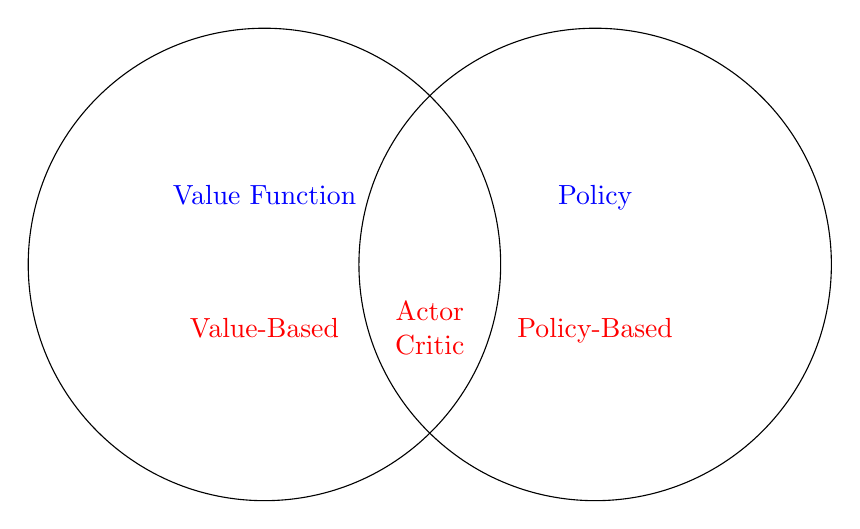
\begin{tikzpicture}
    \draw (0,0) circle (3cm) node {
        \begin{tabular}{c}
            \color{blue}{Value Function} \\
            \\
            \\
            \\
            \color{red}{Value-Based}
        \end{tabular}
    };
    \draw (0:2.1cm) node {
        \begin{tabular}{c}
            \\
            \\
            \\
            \\
            \color{red}{Actor} \\
            \color{red}{Critic}
        \end{tabular}
    };
    \draw (0:4.2cm) circle (3cm) node {
        \begin{tabular}{c}
            \color{blue}{Policy} \\
            \\
            \\
            \\
            \color{red}{Policy-Based}
        \end{tabular}
    };
\end{tikzpicture}

\subsection{Policy-Based RL}\label{subsec:policy-based-rl}
\begin{itemize}
    \item [\textbf{Advantages}]
    \item Better convergence properties than value-based RL.
    \item Effective in high-dimensional state spaces or continuous state spaces.
    \item Can learn stochastic policies.
    \item [\textbf{Disadvantages}]
    \item Typically don't find globally optimum.
    \item Can be inefficient and high variance.
\end{itemize}

\subsection{Policy Optimization}\label{subsec:policy-optimization}
% WARN maybe BAD
%\[
%    \pi_\theta(a|s) = \frac{\exp\left(\frac{Q(s,a,\theta)}{\tau}\right)}{\sum_{a'\in\mathcal{A}}\exp\left(\frac{Q(s,a',\theta)}{\tau}\right)}
%\]

\subsubsection{Policy Gradient}\label{subsubsec:policy-gradient}
% WARN maybe BAD
%\[
%    \nabla_\theta J(\theta) = \mathbb{E}_{\pi_\theta}\left[\sum_{t=0}^{\infty}\nabla_\theta\log\pi_\theta(A_t|S_t)G_t\right]
%\]


AIBO Walk Policies

\subsection{Score Function}\label{subsec:score-function}
Likelihod Ratios
%\[
%    \nabla_\theta J(\theta) = \mathbb{E}_{\pi_\theta}\left[\sum_{t=0}^{\infty}\nabla_\theta\log\pi_\theta(A_t|S_t)G_t\right]
%\]

\subsection{Softmax Policy}\label{subsec:softmax-policy}

\subsection{Gaussian Policy}\label{subsec:gaussian-policy}

\subsection{One Step MDPs}\label{subsec:one-step-mdps}

\subsection{REINFORCE}\label{subsec:reinforce}


%%%%%%%%%%%%%%%%%%%%%%%%%%%%%%%%%%%%%%%%%%%%%%%%%%%%%%%%%%%%%%%%%%%%%%%%%%%%%%%
%%% Experiments
%%%%%%%%%%%%%%%%%%%%%%%%%%%%%%%%%%%%%%%%%%%%%%%%%%%%%%%%%%%%%%%%%%%%%%%%%%%%%%%


\chapter{Experiments}\label{ch:experiments}


%%%%%%%%%%%%%%%%%%%%%%%%%%%%%%%%%%%%%%%%%%%%%%%%%%%%%%%%%%%%%%%%%%%%%%%%%%%%%%%
%%% Exisiting Approaches
%%%%%%%%%%%%%%%%%%%%%%%%%%%%%%%%%%%%%%%%%%%%%%%%%%%%%%%%%%%%%%%%%%%%%%%%%%%%%%%


\chapter{Existing Approaches to Portfolio Allocation}\label{ch:existing-approaches-to-portfolio-allocation}
TODO


\section{Introduction}\label{sec:introduction}
TODO


%%%%%%%%%%%%%%%%%%%%%%%%%%%%%%%%%%%%%%%%%%%%%%%%%%%%%%%%%%%%%%%%%%%%%%%%%%%%%%%
%%% Environment
%%%%%%%%%%%%%%%%%%%%%%%%%%%%%%%%%%%%%%%%%%%%%%%%%%%%%%%%%%%%%%%%%%%%%%%%%%%%%%%


\chapter{Environment}\label{ch:environment}
TODO


\section{Stock Market Environment}\label{sec:stock-market-environment}
TODO

\subsection{Used Frameworks}\label{subsec:used-frameworks}


%%%%%%%%%%%%%%%%%%%%%%%%%%%%%%%%%%%%%%%%%%%%%%%%%%%%%%%%%%%%%%%%%%%%%%%%%%%%%%%
%%% Data
%%%%%%%%%%%%%%%%%%%%%%%%%%%%%%%%%%%%%%%%%%%%%%%%%%%%%%%%%%%%%%%%%%%%%%%%%%%%%%%


\chapter{Data Engineering}\label{ch:data-engineering}
TODO


\section{Data Collection}\label{sec:data-collection}
TODO


\section{Data Preprocessing}\label{sec:data-preprocessing}
TODO

\subsection{Data Cleaning}\label{subsec:data-cleaning}
TODO


\section{Different kinds of Data}\label{sec:different-kinds-of-data}
TODO

\subsection{Fundamental Data}\label{subsec:fundamental-data}
TODO

\subsection{Market Data}\label{subsec:market-data}
TODO

\subsection{Analytics Data}\label{subsec:analytics-data}
TODO

\subsection{Alternative Data}\label{subsec:alternative-data}
TODO


%%%%%%%%%%%%%%%%%%%%%%%%%%%%%%%%%%%%%%%%%%%%%%%%%%%%%%%%%%%%%%%%%%%%%%%%%%%%%%%
%%% Getting Ready Agent
%%%%%%%%%%%%%%%%%%%%%%%%%%%%%%%%%%%%%%%%%%%%%%%%%%%%%%%%%%%%%%%%%%%%%%%%%%%%%%%


\chapter{Agent}\label{ch:agent}
TODO


\section{Training Agent}\label{sec:training-agent}
TODO


\section{Testing Agent}\label{sec:testing-agent}
TODO


\section{Benchmarks and Results}\label{sec:benchmarks-and-results}
TODO


\section{Backtesting}\label{sec:backtesting}
TODO


\section{Portfolio Performance}\label{sec:portfolio-performance}
TODO


%%%%%%%%%%%%%%%%%%%%%%%%%%%%%%%%%%%%%%%%%%%%%%%%%%%%%%%%%%%%%%%%%%%%%%%%%%%%%%%
%%% Contribution to Finrl-Meta
%%%%%%%%%%%%%%%%%%%%%%%%%%%%%%%%%%%%%%%%%%%%%%%%%%%%%%%%%%%%%%%%%%%%%%%%%%%%%%%


\chapter{Contribution to Finrl-Meta}\label{ch:contribution-to-finrl-meta}
TODO


\section{1}\label{sec:1}
TODO

%%%%%%%%%%%%%%%%%%%%%%%%%%%%%%%%%%%%%%%%%%%%%%%%%%%%%%%%%%%%%%%%%%%%%%%%%%%%%%%
%%% Evaluation
%%%%%%%%%%%%%%%%%%%%%%%%%%%%%%%%%%%%%%%%%%%%%%%%%%%%%%%%%%%%%%%%%%%%%%%%%%%%%%%


\chapter{Evaluation}\label{ch:evaluation}
TODO


\section{1}\label{sec:12}
TODO

%%%%%%%%%%%%%%%%%%%%%%%%%%%%%%%%%%%%%%%%%%%%%%%%%%%%%%%%%%%%%%%%%%%%%%%%%%%%%%%
%%% Conclusion
%%%%%%%%%%%%%%%%%%%%%%%%%%%%%%%%%%%%%%%%%%%%%%%%%%%%%%%%%%%%%%%%%%%%%%%%%%%%%%%


\chapter{Conclusion}\label{ch:conclusion}
TODO

\fi
